\documentclass{beamer}

\mode<presentation>
\usetheme{Warsaw}

\usepackage[OT2]{fontenc}
\usepackage{amsfonts}
\usepackage{amssymb}
\usepackage{amsthm}
\usepackage{amsmath}
\usepackage{newlfont}
\usepackage{graphicx}
\usepackage{multicol}
\usepackage[OT2]{fontenc}
\usepackage{wrapfig}
\usepackage{subcaption}
\usepackage{glossaries}
\usepackage{lipsum}
\usepackage[all,arc]{xy}
\usepackage{epsfig}
\usepackage{pgf}
\usepackage{amscd}
\def \zn{,\kern-0.09em,}
\setlength\intextsep{0pt}
\newcommand\texteng{\fontencoding{OT1}\fontfamily{\rmdefault}\selectfont}
\def\ug{\mathbin{\sphericalangle\,}}
\def\dj{d\kern-0.4em\char"16\kern-0.1em}
\def\Dj{\mbox{\raise0.3ex\hbox{-}\kern-0.4em D}}
\newcommand{\D}{\displaystyle}

\title{Geometrijske nejednakosti}
\author{Aleksa Vuchkovic1}
\institute{Matematichka gimnazija}

\date{Mart 2019.}

\setbeamercolor{uppercol}{fg=white,bg=green!75!blue}

\begin{document}

\begin{frame}{}
    \titlepage
    \begin{center}
        \emph{Mentor:} Branko Grbic1, Regionalni centar za talente \zn Mihajlo Pupin'' Panchevo
    \end{center}
\end{frame}
%\maketitle
\begin{frame}
\frametitle{Sadrzhaj}
\tableofcontents
\end{frame}

\section{Geometrijske nejednakosti}
\subsection{Uvod}
\begin{frame}{Uvod}
\onslide<1->
 Pod \textbf{geometrijskom nejednakosh{}c1u} se najchesh{}c1e podrazumeva ona nejednakost koja vazhi za elemente(stranice, uglove, tezhishne duzhi,...) proizvoljnog trougla ili neke slozhenije figure(chetvorougla...). U shirem smislu geometrijska je svaka nejednakost koja se odnosi na neku konkretnu geometrijsku sliku.\\
 \onslide<2->
 \begin{block}{Osnovna nejednakost trougla}
 \centering $a+b>c \quad b+c>a\quad c+a>b$
\end{block}
\end{frame}
\subsection{Osnovne nejednakosti trougla}
\begin{frame}{Osnovne nejednakosti trougla}
\onslide<1->
    \begin{block}{Teorema 1.}
    Naspram vec1e stranice u trouglu je vec1i ugao tog trougla; i obratno, naspram vec1eg ugla trougla je vec1a stranica.
    \end{block}
    \vspace{0.5cm}
    \onslide<2->
\centering   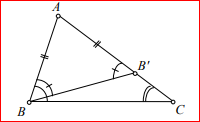
\includegraphics[]{Slika1}
    
\end{frame}
\begin{frame}{Osnovne nejednakosti trougla}
\onslide<1->
   \begin{block}{Teorema 2.}
    (Nejednakost trougla) Zbir dve ivice trougla vec1i je od trec1e.
    \end{block}
    \vspace{0.5cm}
    \onslide<2->
 \centering   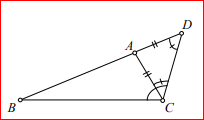
\includegraphics[]{Slika2}
\end{frame}

\section{Ptolomejeva nejednakost}
\begin{frame}{Ptolomejeva nejednakost}
    \onslide<1->
    \begin{block}{Definicija}
    Neka su $A,B,C,D$ bilo koje chetiri tachke u ravni. Tada vazhi nejednakost $$AB\cdot CD+AD\cdot BC \geq AC\cdot BD.$$
    \end{block}
    \onslide<2->
    \begin{block}{Jednakost}
    Jednakost vazhi akko je chetvorougao $ABCD$ tetivni sa dijagonalama $AC$ i $BD$ ili su tachke $A,B,C,D$ kolinearne pri chemu jedna od tachaka $B$ i $D$ lezhi izhmedju tachaka $A$ i $C$, a druga ne.
    \end{block}
\end{frame}

\subsection{Dokaz Ptolomejeve nejednakosti}
\begin{frame}{Dokaz inverzijom}
    \centering   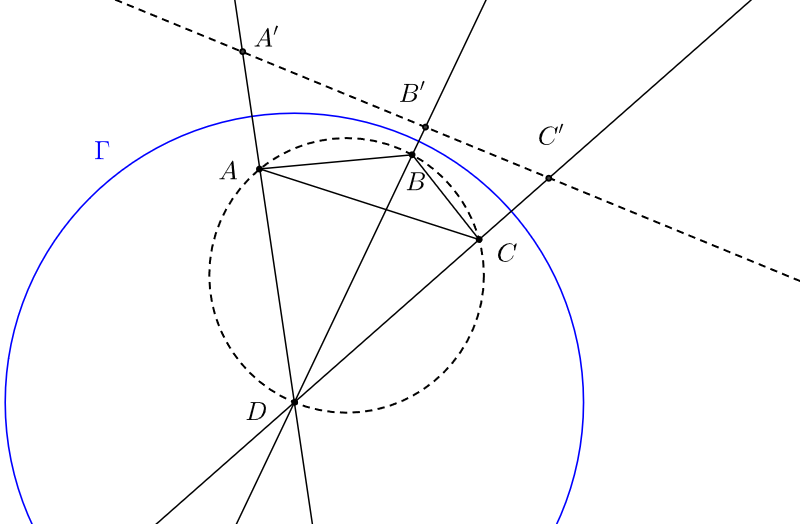
\includegraphics[scale=0.3]{Ptolomej.png}
\end{frame}

\subsection{Primena Ptolomejeve nejednakosti}
\begin{frame}{Primena Ptolomejeve nejednakosti}
    
\begin{block}{Zadatak 1.}
\onslide<1->
Dokazati da vazhi: $\D t_a<\frac{b+c}{2}$
\end{block}
\onslide<2->
\par
\begin{wrapfigure}{r}{0.4\textwidth} %this figure will be at the right
    \centering
    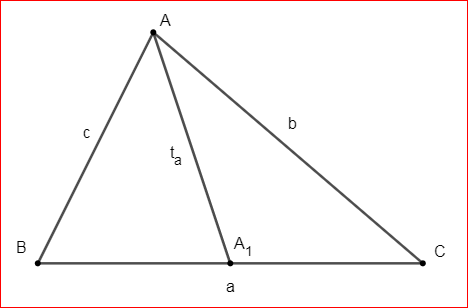
\includegraphics[scale=0.4]{Slika8}
    %\caption*{Slika 5.}
\end{wrapfigure}
Primenjujuc1i Ptolomejevu nejednakost na chetvorougao $ABA_1C$ dobijamo
$AB\cdot A_1C+BA_1\cdot CA>BC\cdot AA_1$, odnosno $\D c\cdot\frac{a}{2}+\frac{a}{2}\cdot b>a\cdot t_a$, shto je ekvivalentno trazhenoj nejednakosti.

\end{frame}

\begin{frame}{Primena Ptolomejeve nejednakosti}
\onslide<1->
    \begin{block}{Zadatak 2.}
    Dokazati da vazhi: $\D 2P\leq bc$
    \end{block}
    \onslide<2->
\begin{wrapfigure}{r}{0.5\textwidth} %this figure will be at the right
   \centering
    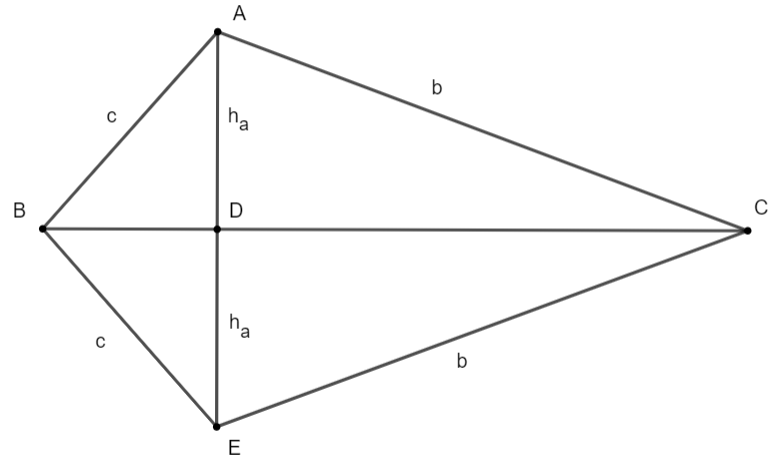
\includegraphics[scale=0.35]{Slika91}
    %\caption*{Slika 5.}
\end{wrapfigure}
    Primenom Ptolomejeve nejednakosti na chetvorougao $ABDC$ dobija se $bc+bc\leq 2ah_a$, iz chega sledi trazhena nejednakost.
\end{frame}

\begin{frame}{Primena Ptolomejeve nejednakosti}
\onslide<1->
    \begin{block}{Zadatak 3.}
    Dokazati da vazhi: $\D l_a<\frac{2bc}{b+c}$ (gde je $l_a$ odsechak bisektrise)
    \end{block}
    \onslide<2->
    \begin{wrapfigure}{r}{0.5\textwidth} %this figure will be at the right
   \centering
    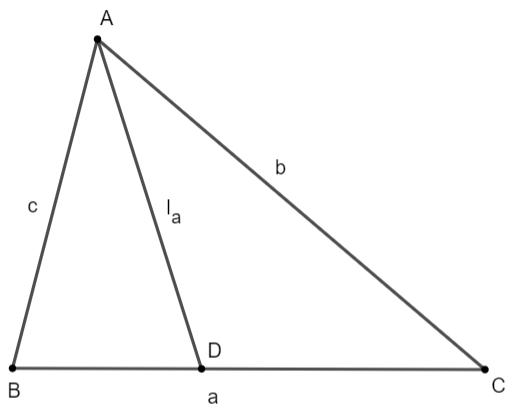
\includegraphics[scale=0.36]{Slika12}
    %\caption*{Slika 5.}
\end{wrapfigure}
    Primenom Ptolomejeve teoreme na chetvorougao $ABDC$ dobijamo $\D AB\cdot DC+BD\cdot CA>BC\cdot AD$, shto daljim postupkom svodimo na trazhenu nejednakost.
\end{frame}

\section{Nejednakosti izmedju sredina}
\begin{frame}{Nejednakosti izmedju sredina}

\begin{block}{Nejednakosti izmedju sredina za $a$ i $b$:}
\centering $\D\frac{2}{\frac{1}{a}+\frac{1}{b}}\leq\sqrt{ab}\leq\frac{a+b}{2}\leq\sqrt{\frac{a^2+b^2}{2}}$.
\end{block}
\centering
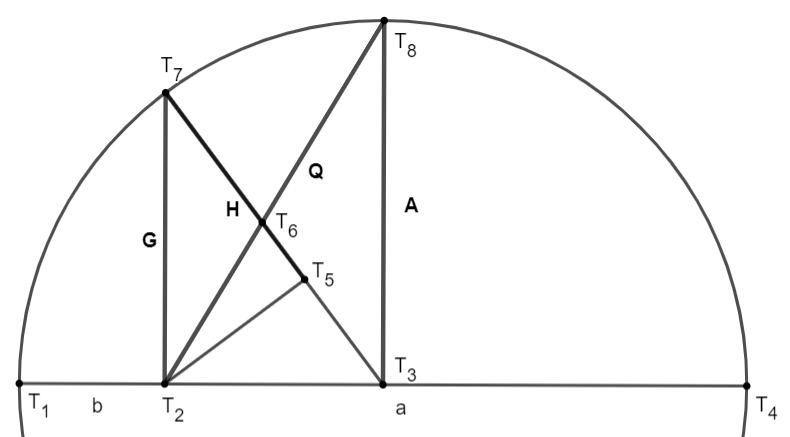
\includegraphics[scale=0.35]{NZM}
\end{frame}


\section{Ojlerova nejednakost}
\begin{frame}{Ojlerova nejednakost}
    \begin{block}{Teorema}
    Ako su $R$ i $r$, redom, poluprechnici opisane i upisane kruzhnice trougla, tada vazhi $R\geq 2r.$
    \end{block}
    \begin{block}{}
    Tvrdjenje se mozhe dokazati i primenom Ojlerovog identiteta, $OI^2 = R^2 - 2Rr$, gde su $O$ i $I$ centri opisane i upisane kruzhnice datog trougla
    \end{block}
\end{frame}

\begin{frame}
 \centering\LARGE   Hvala na pazhnji!
\end{frame}
\end{document}